\documentclass[english]{SPFShortReport}
\usepackage{subfigure}
\usepackage{spfFigures}
\usepackage{longtable}
\usepackage{url}
\usepackage{gensymb}
\usepackage[yyyymmdd,hhmmss]{datetime}
\reportName{Python calculation for heat pump SIN-35TU}
\reportSubName{Parametric Heat Pump calculation} 
\reportDate{\today \hspace{0.1cm} at: \currenttime \hspace{0.1cm} h} 
\author{Dani Carbonell}
\address{dani.carbonell@solarenergy.ch}
\begin{document}
\begin{table}[!ht]
\begin{small}
\caption{Fitted coefficients for the heat pump.}
\begin{center}
\resizebox{12cm}{!} 
{
\begin{tabular}{l | c c } 
\hline
\hline
Coefficient &Description & \\ 
 & &$[kW]$\\ 
\hline
$PQ_{1}$ & \emph{$1^{st}$ condenser polynomial coefficient}  & 3.5066e+01    \\ 
$PQ_{2}$ & \emph{$2^{st}$ condenser polynomial coefficient}  & 3.8459e+02    \\ 
$PQ_{3}$ & \emph{$3^{st}$ condenser polynomial coefficient}  & 6.5501e+01    \\ 
$PQ_{4}$ & \emph{$4^{st}$ condenser polynomial coefficient}  & -6.2781e+02    \\ 
$PQ_{5}$ & \emph{$5^{st}$ condenser polynomial coefficient}  & 3.8715e+02    \\ 
$PQ_{6}$ & \emph{$6^{st}$ condenser polynomial coefficient}  & -3.7043e+02    \\ 
\hline
$PCOP_{1}$ & \emph{$1^{st}$ COP polynomial coefficient}  & 7.5227e+01    \\ 
$PCOP_{2}$ & \emph{$2^{st}$ COP polynomial coefficient}  & 1.8270e+02    \\ 
$PCOP_{3}$ & \emph{$3^{st}$ COP polynomial coefficient}  & -9.8056e+02    \\ 
$PCOP_{4}$ & \emph{$4^{st}$ COP polynomial coefficient}  & -7.3151e+02    \\ 
$PCOP_{5}$ & \emph{$5^{st}$ COP polynomial coefficient}  & -2.9248e+03    \\ 
$PCOP_{6}$ & \emph{$6^{st}$ COP polynomial coefficient}  & 3.3858e+03    \\ 
\hline
$\dot m_{cond}$ & 6100.00 $[kg/h]$\\ 
$\dot m_{evap}$ & 6100.00 $[kg/h]$\\ 
\hline
$COP_{nom}$ (B0W35)& 5.50 \\ 
$Q_{c,nom}$ (B0W35)& 35.12 kW\\ 
$COP_{nom}$ (B2W35)& 6.41 \\ 
$Q_{c,nom}$ (B2W35)& 37.14 kW\\ 
$COP_{nom}$ (B10W35)& 7.57 \\ 
$Q_{c,nom}$ (B10W35)& 45.82 kW\\ 
\hline
\hline
\end{tabular}
}
\label{CoefTable}
\end{center}
\end{small}
\end{table}
\begin{table}[!ht]
\begin{small}
\caption{Predicting results of the heat pump.}
\begin{center}
\resizebox{12cm}{!} 
{
\begin{tabular}{l | c c c c c c c c c c c } 
\hline
\hline
$T_{evap,in}$ &$T_{evap,out}$ &$T_{cond,in}$ &$T_{cond,out}$ &$COP$ &$Q_{cond}$ &$Q_{evap}$ &$W_{comp}$ &$\dot m_{cond}$ &$\dot m_{evap}$ &$\Delta T_{evap}$ &$\Delta T_{cond}$ \\ 
$^oC$ &$^oC$ &$^oC$ &$^oC$ &$[-]$ &$[kW]$ &$[kW]$ &$[kW]$ &kg/h &kg/h &K &K\\ 
\hline
-7.00 & -10.25 & 26.03 & 30.00 & 3.95 & 28.16 & 21.04 & 7.12 & 6100 & 6100 & 3.3 & 4.0\\ 
-7.00 & -12.88 & 34.98 & 38.75 & -2.37 & 26.76 & 38.04 & -11.28 & 6100 & 6100 & 5.9 & 3.8\\ 
-7.00 & -14.67 & 43.95 & 47.50 & -1.03 & 25.17 & 49.60 & -24.42 & 6100 & 6100 & 7.7 & 3.5\\ 
-7.00 & -29.20 & 53.74 & 56.25 & -0.14 & 17.83 & 143.57 & -125.74 & 6100 & 6100 & 22.2 & 2.5\\ 
-7.00 & -10.44 & 61.75 & 65.00 & 26.59 & 23.09 & 22.22 & 0.87 & 6100 & 6100 & 3.4 & 3.3\\ 
-4.00 & -8.07 & 25.63 & 30.00 & 6.66 & 31.00 & 26.34 & 4.65 & 6100 & 6100 & 4.1 & 4.4\\ 
-4.00 & -6.41 & 34.30 & 38.75 & 1.97 & 31.61 & 15.56 & 16.05 & 6100 & 6100 & 2.4 & 4.5\\ 
-4.00 & -7.24 & 43.26 & 47.50 & 3.28 & 30.12 & 20.93 & 9.20 & 6100 & 6100 & 3.2 & 4.2\\ 
-4.00 & -7.96 & 52.31 & 56.25 & 11.86 & 27.95 & 25.59 & 2.36 & 6100 & 6100 & 4.0 & 3.9\\ 
-4.00 & -7.79 & 61.42 & 65.00 & 27.98 & 25.40 & 24.49 & 0.91 & 6100 & 6100 & 3.8 & 3.6\\ 
-1.00 & -5.68 & 25.21 & 30.00 & 8.95 & 34.04 & 30.23 & 3.80 & 6100 & 6100 & 4.7 & 4.8\\ 
-1.00 & -4.75 & 33.95 & 38.75 & 3.47 & 34.09 & 24.28 & 9.81 & 6100 & 6100 & 3.8 & 4.8\\ 
-1.00 & -4.97 & 42.89 & 47.50 & 4.65 & 32.74 & 25.70 & 7.04 & 6100 & 6100 & 4.0 & 4.6\\ 
-1.00 & -5.36 & 51.95 & 56.25 & 13.00 & 30.53 & 28.18 & 2.35 & 6100 & 6100 & 4.4 & 4.3\\ 
-1.00 & -5.15 & 61.08 & 65.00 & 28.74 & 27.80 & 26.84 & 0.97 & 6100 & 6100 & 4.2 & 3.9\\ 
2.00 & -3.21 & 24.76 & 30.00 & 10.70 & 37.20 & 33.72 & 3.48 & 6100 & 6100 & 5.2 & 5.2\\ 
2.00 & -2.50 & 33.54 & 38.75 & 4.68 & 36.97 & 29.07 & 7.90 & 6100 & 6100 & 4.5 & 5.2\\ 
2.00 & -2.50 & 42.49 & 47.50 & 5.52 & 35.55 & 29.10 & 6.44 & 6100 & 6100 & 4.5 & 5.0\\ 
2.00 & -2.76 & 51.57 & 56.25 & 13.53 & 33.20 & 30.75 & 2.45 & 6100 & 6100 & 4.8 & 4.7\\ 
2.00 & -2.52 & 60.73 & 65.00 & 28.88 & 30.29 & 29.24 & 1.05 & 6100 & 6100 & 4.5 & 4.3\\ 
5.00 & -0.73 & 24.30 & 30.00 & 11.89 & 40.46 & 37.06 & 3.40 & 6100 & 6100 & 5.7 & 5.7\\ 
5.00 & -0.04 & 33.11 & 38.75 & 5.37 & 40.05 & 32.59 & 7.46 & 6100 & 6100 & 5.0 & 5.6\\ 
5.00 & 0.07 & 42.08 & 47.50 & 5.81 & 38.50 & 31.86 & 6.63 & 6100 & 6100 & 4.9 & 5.4\\ 
5.00 & -0.15 & 51.18 & 56.25 & 13.45 & 35.97 & 33.30 & 2.67 & 6100 & 6100 & 5.1 & 5.1\\ 
5.00 & 0.10 & 60.37 & 65.00 & 28.40 & 32.87 & 31.71 & 1.16 & 6100 & 6100 & 4.9 & 4.6\\ 
8.00 & 1.76 & 23.83 & 30.00 & 12.52 & 43.82 & 40.32 & 3.50 & 6100 & 6100 & 6.2 & 6.2\\ 
8.00 & 2.53 & 32.66 & 38.75 & 5.50 & 43.27 & 35.40 & 7.87 & 6100 & 6100 & 5.5 & 6.1\\ 
8.00 & 2.74 & 41.64 & 47.50 & 5.49 & 41.59 & 34.01 & 7.58 & 6100 & 6100 & 5.3 & 5.9\\ 
8.00 & 2.46 & 50.78 & 56.25 & 12.76 & 38.83 & 35.79 & 3.04 & 6100 & 6100 & 5.5 & 5.5\\ 
8.00 & 2.71 & 60.00 & 65.00 & 27.30 & 35.53 & 34.23 & 1.30 & 6100 & 6100 & 5.3 & 5.0\\ 
11.00 & 4.27 & 23.34 & 30.00 & 12.59 & 47.27 & 43.51 & 3.76 & 6100 & 6100 & 6.7 & 6.7\\ 
11.00 & 5.22 & 32.18 & 38.75 & 5.02 & 46.67 & 37.37 & 9.30 & 6100 & 6100 & 5.8 & 6.6\\ 
11.00 & 5.60 & 41.18 & 47.50 & 4.51 & 44.88 & 34.94 & 9.94 & 6100 & 6100 & 5.4 & 6.3\\ 
11.00 & 5.10 & 50.36 & 56.25 & 11.45 & 41.80 & 38.15 & 3.65 & 6100 & 6100 & 5.9 & 5.9\\ 
11.00 & 5.31 & 59.61 & 65.00 & 25.58 & 38.29 & 36.79 & 1.50 & 6100 & 6100 & 5.7 & 5.4\\ 
14.00 & 6.79 & 22.84 & 30.00 & 12.08 & 50.82 & 46.62 & 4.21 & 6100 & 6100 & 7.2 & 7.2\\ 
14.00 & 8.24 & 31.66 & 38.75 & 3.84 & 50.36 & 37.26 & 13.10 & 6100 & 6100 & 5.8 & 7.1\\ 
14.00 & 9.40 & 40.62 & 47.50 & 2.56 & 48.84 & 29.76 & 19.08 & 6100 & 6100 & 4.6 & 6.9\\ 
14.00 & 7.79 & 49.93 & 56.25 & 9.51 & 44.89 & 40.17 & 4.72 & 6100 & 6100 & 6.2 & 6.3\\ 
14.00 & 7.91 & 59.21 & 65.00 & 23.26 & 41.13 & 39.37 & 1.77 & 6100 & 6100 & 6.1 & 5.8\\ 
17.00 & 9.34 & 22.33 & 30.00 & 11.00 & 54.49 & 49.53 & 4.95 & 6100 & 6100 & 7.7 & 7.7\\ 
17.00 & 13.31 & 31.00 & 38.75 & 1.77 & 54.99 & 23.89 & 31.10 & 6100 & 6100 & 3.7 & 7.7\\ 
17.00 & 13.61 & 40.42 & 47.50 & 1.77 & 50.25 & 21.93 & 28.32 & 6100 & 6100 & 3.4 & 7.1\\ 
17.00 & 10.64 & 49.47 & 56.25 & 6.86 & 48.17 & 41.15 & 7.02 & 6100 & 6100 & 6.4 & 6.8\\ 
17.00 & 10.52 & 58.79 & 65.00 & 20.32 & 44.08 & 41.91 & 2.17 & 6100 & 6100 & 6.5 & 6.2\\ 
20.00 & 11.95 & 21.79 & 30.00 & 9.32 & 58.28 & 52.03 & 6.25 & 6100 & 6100 & 8.0 & 8.2\\ 
20.00 & 15.85 & 30.75 & 38.75 & 1.90 & 56.76 & 26.83 & 29.93 & 6100 & 6100 & 4.1 & 8.0\\ 
20.00 & 16.46 & 40.38 & 47.50 & 1.83 & 50.57 & 22.87 & 27.70 & 6100 & 6100 & 3.5 & 7.1\\ 
20.00 & 15.84 & 48.79 & 56.25 & 2.03 & 52.94 & 26.88 & 26.06 & 6100 & 6100 & 4.2 & 7.5\\ 
20.00 & 13.15 & 58.36 & 65.00 & 16.75 & 47.13 & 44.31 & 2.81 & 6100 & 6100 & 6.9 & 6.6\\ 
\hline
\hline
\end{tabular}
}
\label{ResultsTable}
\end{center}
\end{small}
\end{table}
\begin{figure}[!ht]
\begin{center}
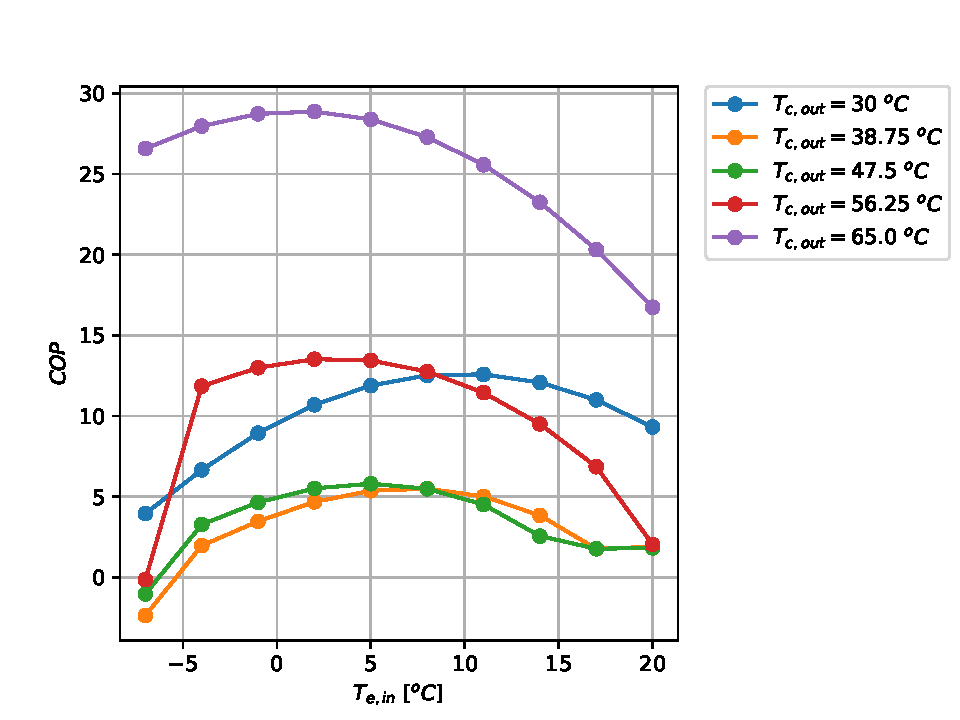
\includegraphics[width=1\textwidth]{C:/Daten/spfPackages/GIT/spfTrnsysFiles/HeatPump/BrineToWater/Walter Meier/SIN-35TU/SIN-35TU-Cop.pdf}
\caption{COP Results for the heat pump at the selected points}
\label{COPFig}
\end{center}
\end{figure}
\begin{figure}[!ht]
\begin{center}
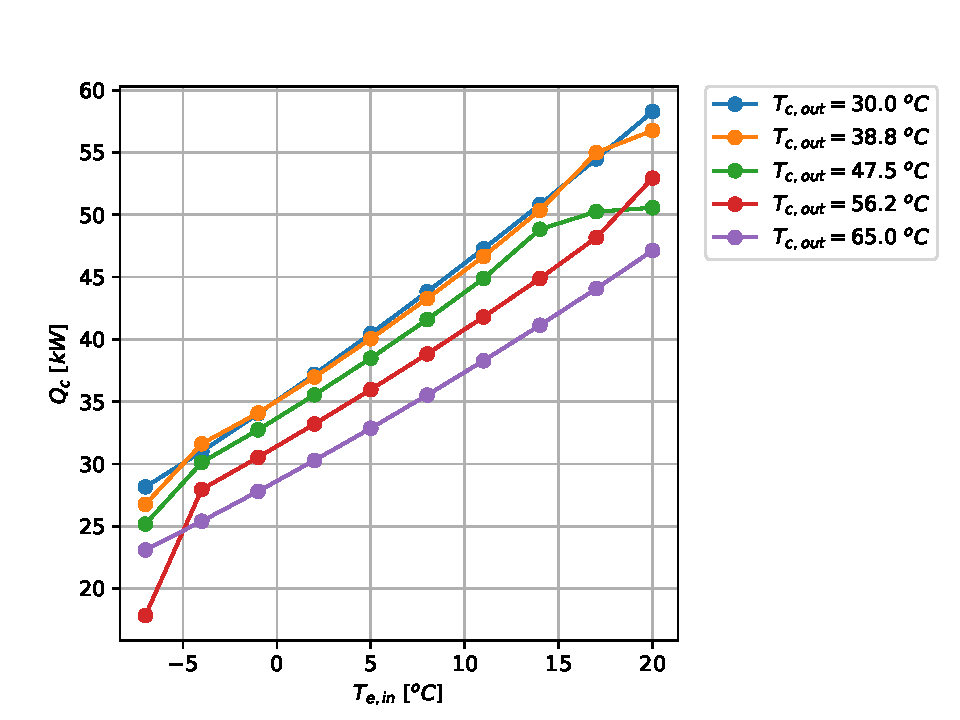
\includegraphics[width=1\textwidth]{C:/Daten/spfPackages/GIT/spfTrnsysFiles/HeatPump/BrineToWater/Walter Meier/SIN-35TU/SIN-35TU-Qc.pdf}
\caption{$Q_c$ Results for the heat pump at the selected points}
\label{QcFig}
\end{center}
\end{figure}
\end{document}
